% Main tex file for the New Trends in Research Colloquium
% Author: Javier Reyes

\documentclass{beamer}

\usetheme{metropolis}
\usefonttheme[onlymath]{serif}
\metroset{subsectionpage=progressbar, sectionpage=none, block=fill}

% Colors for block environments
% \setbeamercolor{block title default}{use=default text,
% 		fg=default text.fg,
% 		bg=default text.bg!80!default text.fg}
% \setbeamercolor{block body default}{use={block title default, default text},
% 		fg=default text.fg,
% 		bg=block title default.bg!90!default text.bg}
% \setbeamercolor{block title alerted}{use=alerted text,
% 		fg=alerted text.fg,
% 		bg=alerted text.bg!80!alerted text.fg}
% \setbeamercolor{block body alerted}{use={block title alerted, alerted text},
% 		fg=alerted text.fg,
% 		bg=block title alerted.bg!90!alerted text.bg}
% \setbeamercolor{block title example}{use=example text,
% 		fg=example text.fg,
% 		bg=example text.bg!80!example text.fg}
% \setbeamercolor{block body example}{use={block title example, example text},
% 		fg=example text.fg,
% 		bg=block title example.bg!90!example text.bg}

% Encoding format
\usepackage[utf8]{inputenc}

% References management
\usepackage[backend=biber,
						citestyle=numeric]{biblatex}
\bibliography{../references.bib}
\setbeamertemplate{bibliography item}{\insertbiblabel}

% Position images
\usepackage[export]{adjustbox}

% Math functions
\usepackage{amsmath}

% Required to insert images
\usepackage{graphicx}
\graphicspath{{pres-img/}}

% Required to use color
\usepackage{color}

% Formated code insertion package
\usepackage{listings}

% Set line spaces
\usepackage{setspace}

\usepackage{hanging}
\setbeamertemplate{footnote}{
  \hangpara{2em}{1}
  \makebox[2em][l]{\insertfootnotemark}\scriptsize\insertfootnotetext\par
}

\usepackage{multicol}

\title{Zynqberry Operator Accelerator Plus}
\subtitle{New Trends in Research}
\author{Javier Ignacio Reyes Garcia \\
	\tiny{\texttt{javier.reyesgarcia001@stud.fh-dortmund.de}}}
\institute{Dortmund University of Applied Sciences and Arts}
\date{\today}

\begin{document}

\maketitle

\begin{frame}{Outline}
	\setbeamertemplate{section in toc}[circle]
	\setbeamertemplate{subsection in toc}[ball unnumbered]
	\begin{columns}[t]
		\begin{column}{.5\textwidth}
				\tableofcontents[sections={1-2}]
		\end{column}
		\begin{column}{.5\textwidth}
				\tableofcontents[sections={3-4}]
		\end{column}
	\end{columns}
\end{frame}

\setbeamertemplate{frame footer}{\tiny{New Trends in Research} \hspace{2cm} \tiny{Dortmund University of Applied Sciences and Arts}}

\section{DAEbot}
% Chapter 1 (from pres-main tex file)
% New Trends in Research
% Author: Javier Reyes

\subsection{DAEbot Project}

\begin{frame}
	\frametitle{DAEbot Project}
	\begin{columns}
		\begin{column}{0.4\textwidth}
			\begin{flushleft}
				\setstretch{1.5}\LARGE
				\textbf{D}istributed \\
				\textbf{A}rchitecture \\
				\textbf{E}valuation \\
				ro\textbf{BOT}
			\end{flushleft}
		\end{column} \pause
		\begin{column}{0.6\textwidth}
			\begin{figure}
				\includegraphics[width=\textwidth]{daebot-pic.png}
				\caption{DAEbot physical chasis, from \cite{Wiki}.}\label{fig:daebot-pic}
			\end{figure}
		\end{column}
	\end{columns}
\end{frame}

\begin{frame}
	\frametitle{DAEbot Project}
	Characteristics\footnote[frame]{See oficial Wiki \cite{Wiki}}:
	\begin{itemize}
		\item Designed to be modular. \pause
		\item Allows different approaches for distributed HW and SW architectures. \pause
		\item Robust and big enough to carry several sensors and actuators.
	\end{itemize}
\end{frame}

\subsection{DAEbot Structure}

\begin{frame}
	\frametitle{DAEbot Structure}
	\begin{figure}
		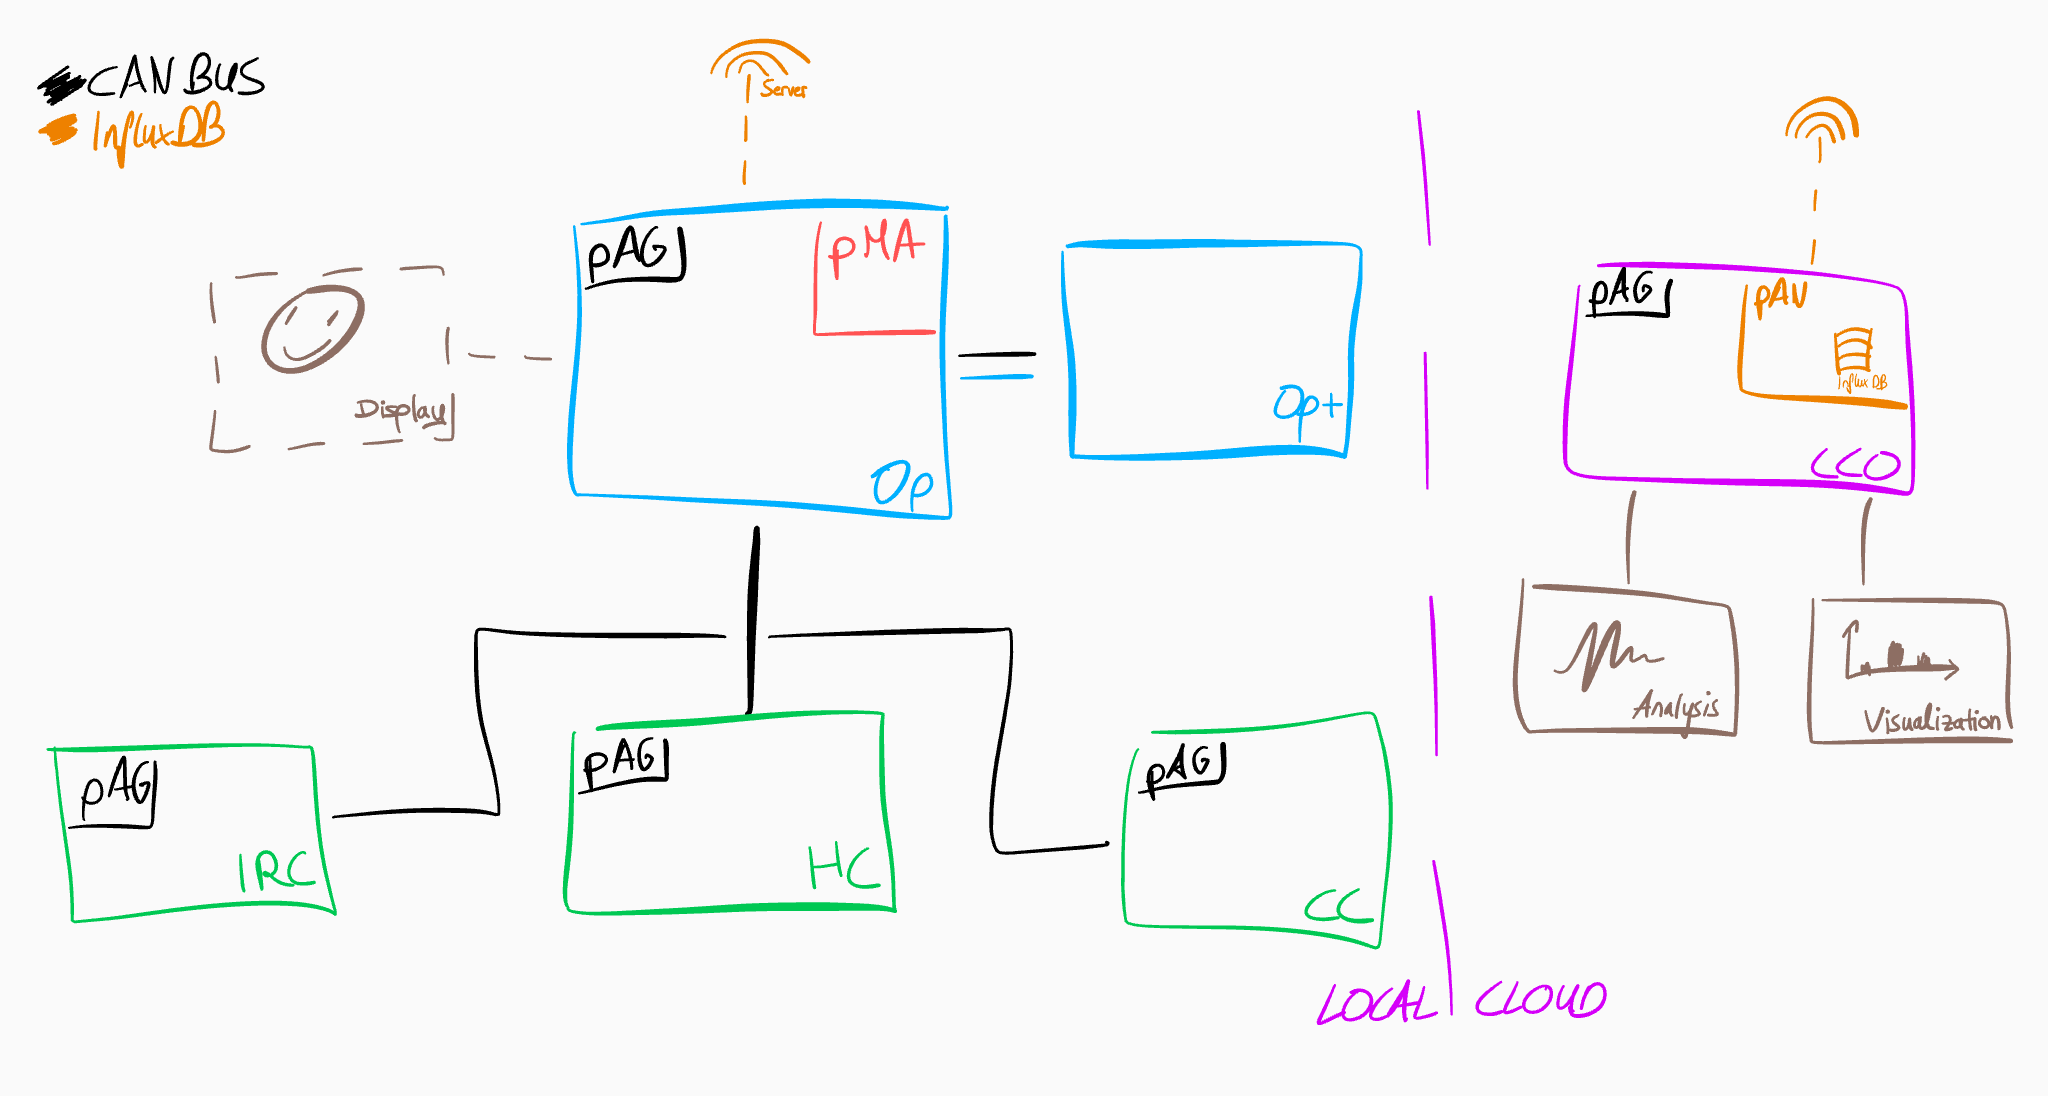
\includegraphics[width=0.7\textwidth, center]{daebot-concept-new.png}
		\caption{DAEbot software concept, from \cite{Wiki}.}\label{fig:daebot-concept-new}
	\end{figure}
\end{frame}

\begin{frame}
	\frametitle{DAEbot Structure}
	\begin{figure}
		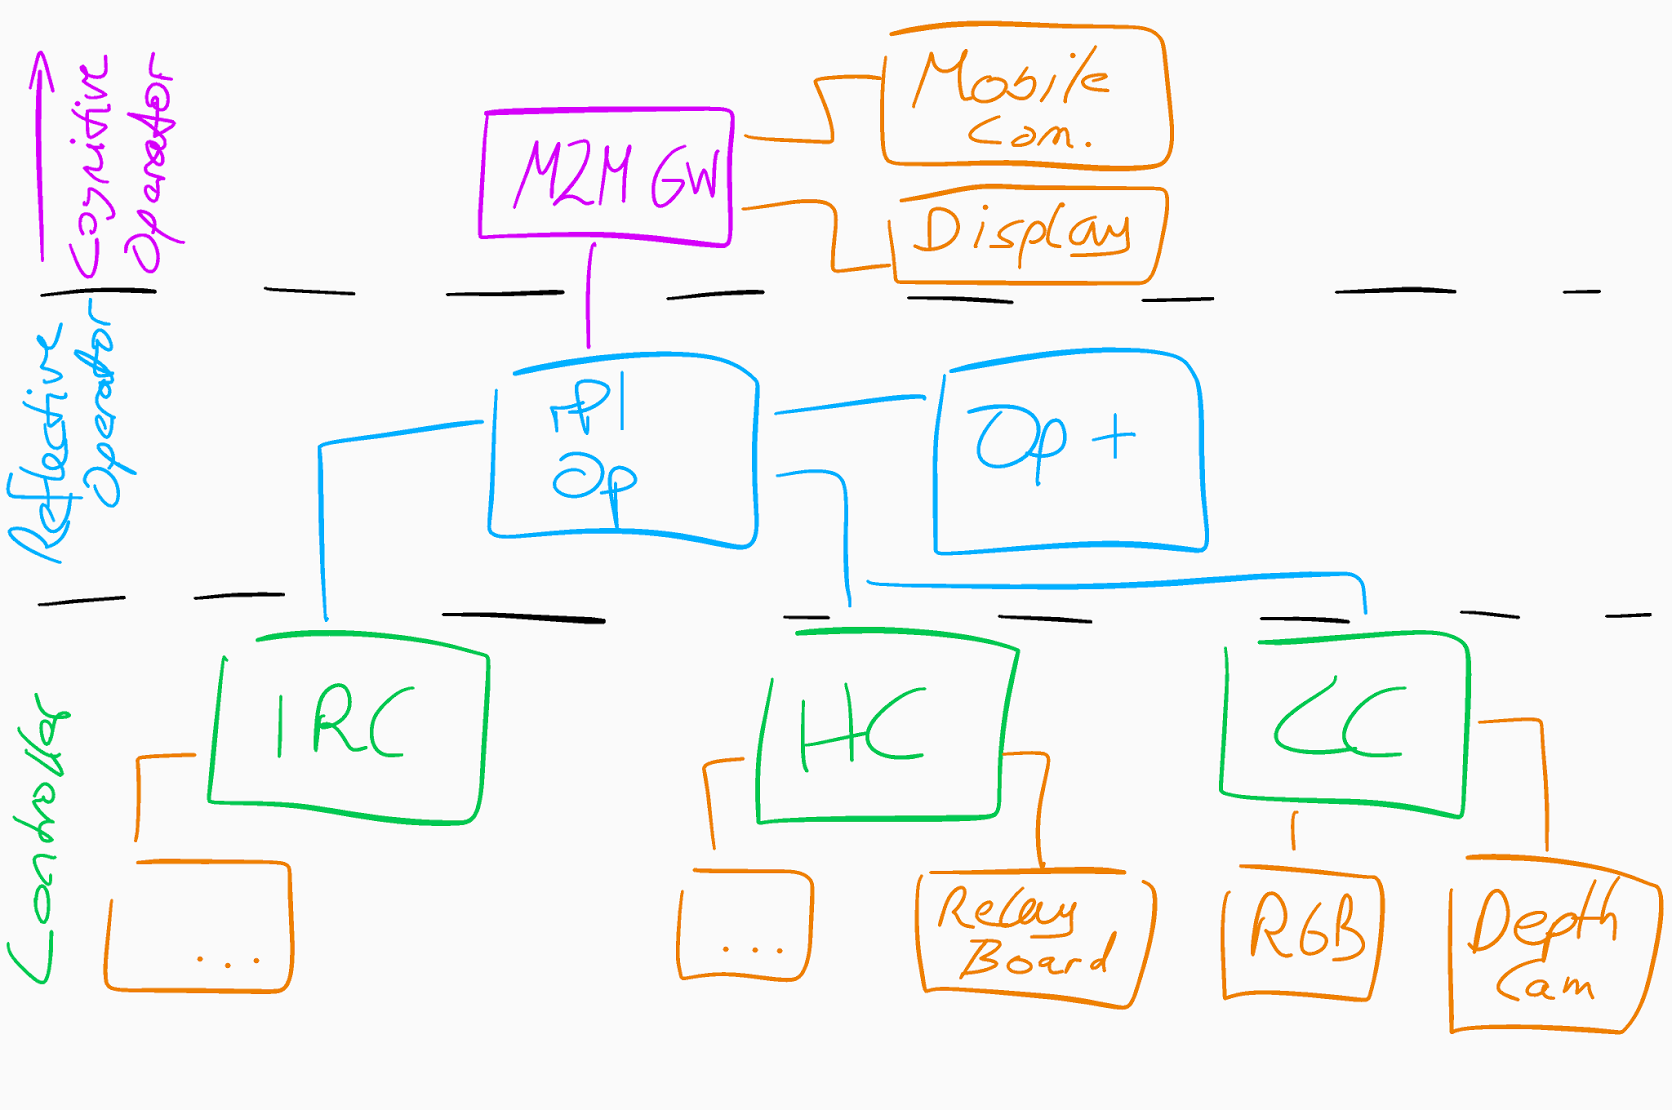
\includegraphics[width=0.7\textwidth, center]{daebot-concept-hand.png}
		\caption{DAEbot architecture, based on OCM concept, from \cite{Wiki}.}\label{fig:daebot-concept-hand}
	\end{figure}
\end{frame}

\subsection{OCM Structure}

\begin{frame}
	\frametitle{OCM Structure}
	Layers\footnote[frame]{See \cite{Lueckel2001}}:
	\begin{itemize}
		\item Controller: Lowest level layer, traditional controller as a \underline{control loop}, usually based on mathematical model. \pause
		\item Reflective Operator: Monitoring and control, allows communication with other systems in a network. \pause
		\item Cognitive Operator: Coordination/communication interactions or learning algorithms, expanded functionality.
	\end{itemize}
\end{frame}

\begin{frame}
	\frametitle{OCM Structure}
	\begin{figure}
		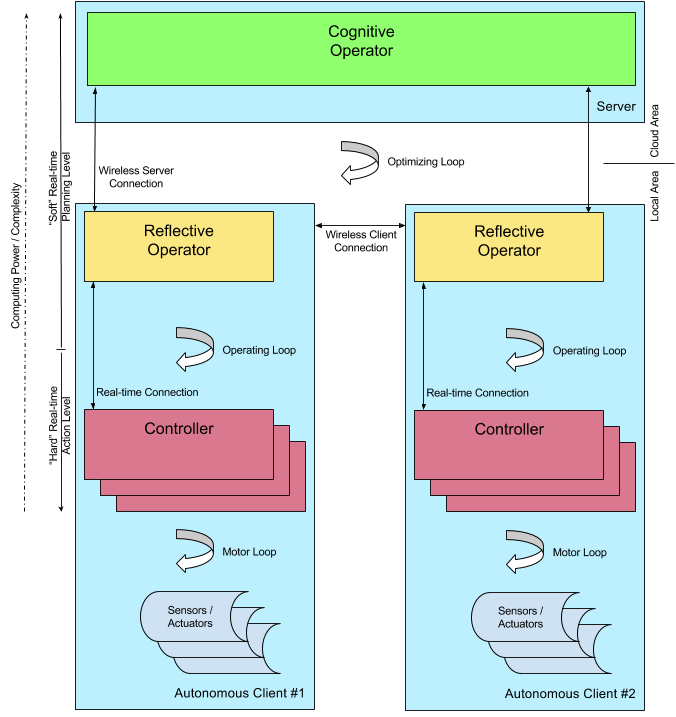
\includegraphics[width=0.5\textwidth, center]{ocm-architecture.png}
		\caption{OCM general structure diagram, from \cite{Wiki}.}\label{fig:ocm-architecture}
	\end{figure}
\end{frame}

\begin{frame}
	\frametitle{DAEbot need}
	\textbf{\LARGE{Operator+ Goal:}} \\
	\large{Provide additional resources for the main Reflective Operator, thanks to its advantages in speed for parallel tasks in FPGA hardware.}
	\vfill \pause
	\begin{exampleblock}{Condition}
		The main Reflective Operator activates (via relay) the Operator+ when it is needed.
	\end{exampleblock}
\end{frame}

\section{Zynqberry SBC}
% Chapter 1 (from pres-main tex file)
% New Trends in Research
% Author: Javier Reyes

\subsection{Zynqberry 726}

\begin{frame}
	\frametitle{Zynqberry 726}
	Single Board Computer:
	\begin{itemize}
		\item Xilinx Zynq-7010 device. \pause
		\item Raspberry Pi Form Factor. \pause
		\item Board-mounted peripherials:
		\begin{itemize}
			\item 16 MB Flash, 512 MB DDR3L SDRAM, 4xUSB 2.0, 10/100 Mbit Ethernet RJ45, Micro SD card slot, HDMI connector, DSI display connector, CSI-2 camera connector, HAT header with 26 IO, 3.5 mm stereo audio socket, Micro-USB (power, USB-UART, JTAG).
		\end{itemize}
	\end{itemize}
\end{frame}

\begin{frame}
	\frametitle{Zynqberry 726}
	\begin{columns}
		\begin{column}{0.4\textwidth}
			\begin{figure}
				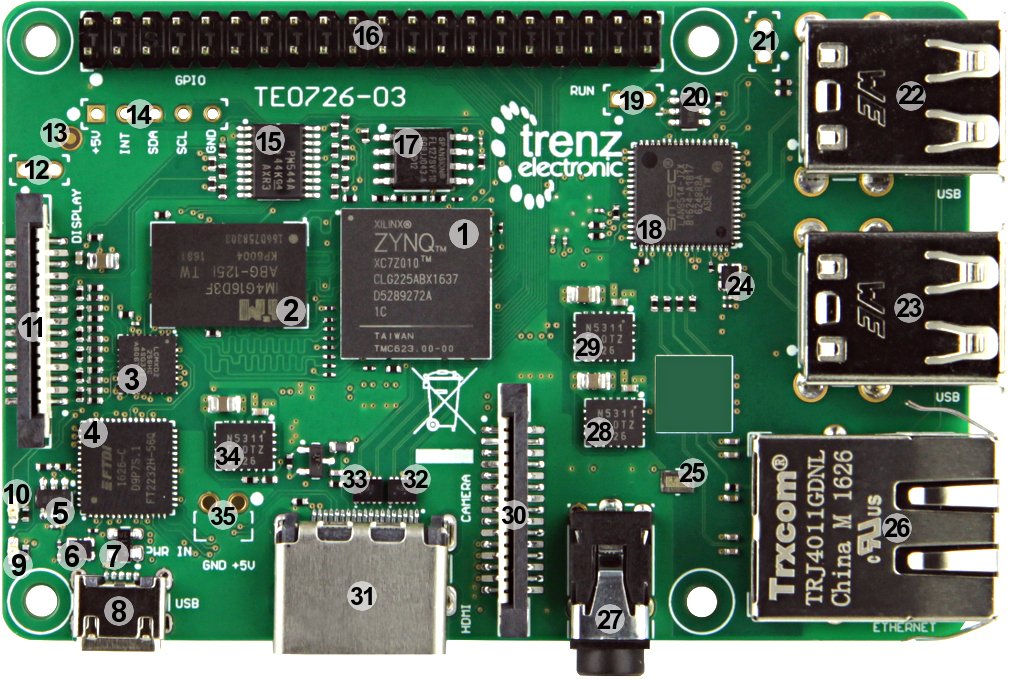
\includegraphics[width=\textwidth]{zynqberry-top.png}
				\caption{Zynqberry 726 board, from \cite{zynq-main}.}\label{fig:zynqberry-top}
			\end{figure}
		\end{column} \pause
		\begin{column}{0.5\textwidth}
			\begin{figure}
				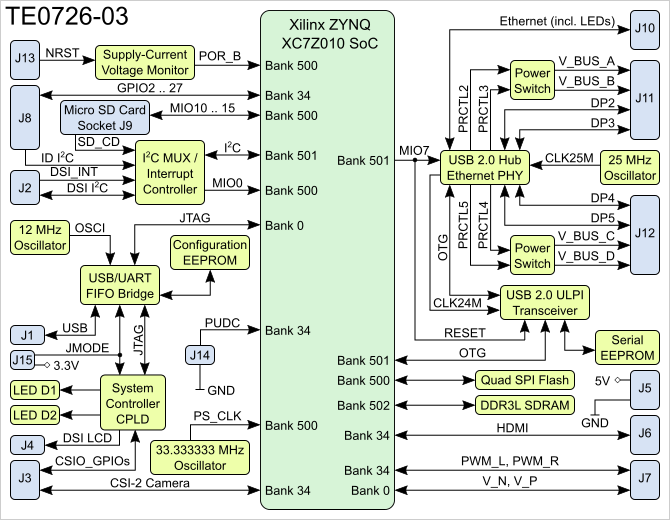
\includegraphics[width=\textwidth]{zynq-block-diagram.png}
				\caption{Zynqberry 726 block diagram, from \cite{zynq-trm}.}\label{fig:zynq-block-diagram}
			\end{figure}
		\end{column}
	\end{columns}
\end{frame}

\subsection{Zynq XC7Z010}

\begin{frame}
	\frametitle{Zynq XC7Z010}
	System on Chip (SoC) device from the Xilinx Zynq 7000 family:
	\begin{itemize}
		\item Dual-core ARM Cortex A9 processor. \pause
		\item 28 nm Xilinx Artix-7 programmable logic device. \pause
		\item Integrated memory mapped Peripherals:
		\begin{itemize}
			\item 2x USB 2.0, 2x Gigabit Ethernet, 2x SD, 2x UART, 2x CAN 2.0B, 2x I2C, 2x SPI, 32b GPIO.
		\end{itemize}
	\end{itemize}
\end{frame}

\begin{frame}
	\frametitle{Zynq 7000 family}
	\begin{figure}
		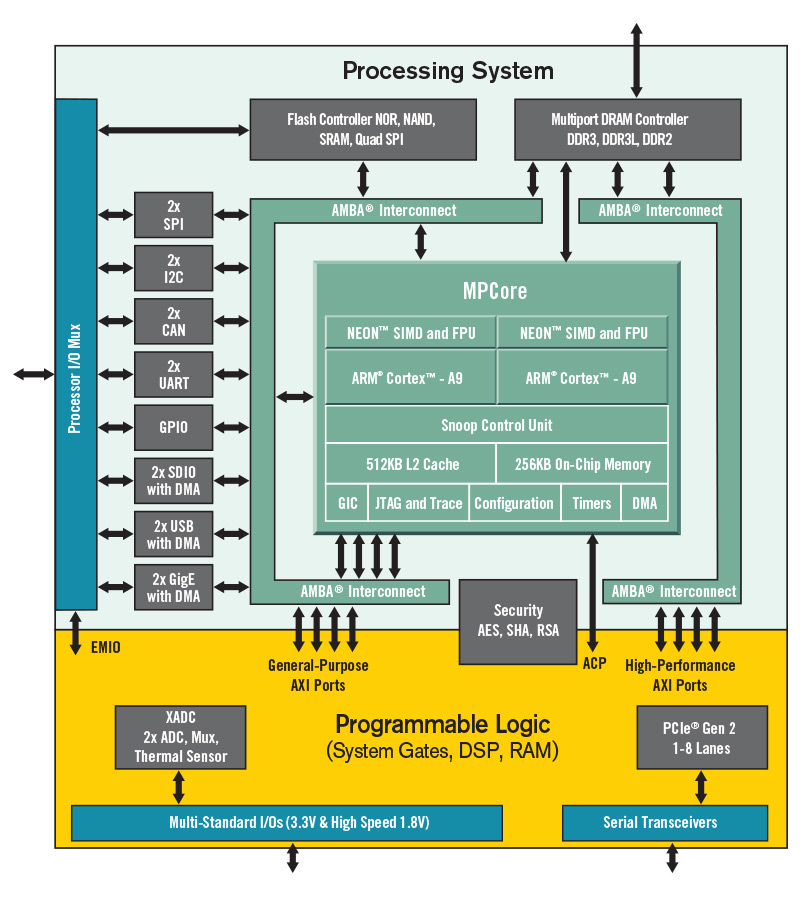
\includegraphics[width=0.4\textwidth]{zynq-arch-diag.png}
		\caption{Zynq-7000 device family architecture, from Xilinx Product Webpage.} \label{fig:zynq-arch-diag}
	\end{figure}
\end{frame}

\begin{frame}
	\frametitle{Zynqberry Vs. Zynq 7Z010}
	The PS includes two Ethernet controllers, but the PHY attached to the Ethernet port on the board is connected to a USB-to-Ethernet interface.
	\vfill \pause
	\begin{alertblock}{Constraint}
		The hardware design needs to use the USB controller for any Ethernet communication.
	\end{alertblock}
\end{frame}

\section{Vivado Design Suite}
% Chapter 1 (from pres-main tex file)
% New Trends in Research
% Author: Javier Reyes

\subsection{Vivado HLx}

\begin{frame}
	\frametitle{Vivado HLx}
	Replacing ISE tools, the tool suite allows design, integration and implementation of systems for the Xilinx technologies.
	\vfill
	Included programs:
	\begin{itemize}
		\item Vivado HLx - High Level design
		\item Xilinx SDK - Software development 
		\item Vivado HLS - High Level Synthesis
		\item (Optional, external) Petalinux - Embedded Linux image building
	\end{itemize}
\end{frame}

\begin{frame}
	\frametitle{Vivado HLx}
	\begin{itemize}
		\item Interaction through GUI or native embedded TCL scripting language (commands either through the IDE console, or as file scripts). 
		\item Runs under Windows and Linux\footnote[frame]{Distro dependant, see \cite{UG973}} OS.
	\end{itemize}
\end{frame}

\begin{frame}
	\frametitle{IDiAL Server}
	Given the high requirements and the need to mantain a common work platform, a Virtual Machine is created in the IDiAL Server, where the tools are available to create/modify the designs.
	\vfill
	\begin{itemize}
		\item VM: U16x64D\_Vivado
		\item User: Javier
		\item Password: IDiAL
		\item OS: Ubuntu 16.04.3 Desktop
		\item IP-Address: 172.22.167.120
	\end{itemize}
\end{frame}

\begin{frame}[fragile]
	\frametitle{Basic install \& launch}
	\begin{lstlisting}[language=bash, basicstyle=\tiny\ttfamily, tabsize=2, commentstyle=\color{darkgray}, keywordstyle=\color{blue}, backgroundcolor=\color{lightgray}, morekeywords={chmod, sudo}, breaklines=true]
# Give executable permission to the installer file
chmod +x <installer_filename>.bin
# Executes the installer with root privileges
# Select the WebPack edition - no cost
# Include at least the SDK and the device Zynq in the content selection
# Select the installation folder
sudo ./<installer_filename>.bin
# After install, change to the driver cable installer folder
cd <vivado_folder>/data/xicom/cable_drivers/lin64/install_script/install_drivers/
# Execute the driver cable installer with root privileges
sudo ./install_drivers
# Create the apropiate environment for the suite to be launched
# Needs to be run everytime before launching Vivado
# Alternatively, can be added to the .bashrc to be executed automatically
source _vivado_installed_folder_/settings64.sh
# Launch the Vivado GUI, blocks the terminal when launched
vivado &
	\end{lstlisting}
	\begin{alertblock}{Constraint}
		{\small The Windows installer runs automatically the USB drivers, while in Linux it needs to be run after the Installation.}
	\end{alertblock}
\end{frame}

\begin{frame}
	\frametitle{Hardware Project}
	\begin{columns}
		\begin{column}{0.5\textwidth}
			\begin{figure}
				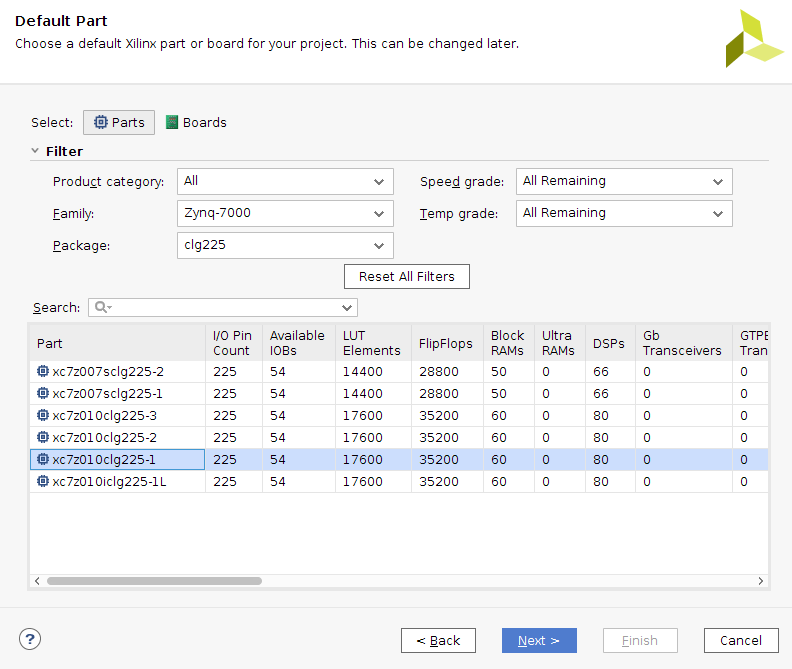
\includegraphics[width=\textwidth]{project-device.png}
				\caption{Vivado project - Device selection.}\label{fig:project-device}
			\end{figure}
		\end{column}
		\begin{column}{0.5\textwidth}
			\begin{itemize}
				\item Create a new project.
				\item Select RTL project type.
				\item Select the correspondent device.
				\item Create a new Block Design.
				\item Add the Zynq7 IP Core.
				\item Add/create any other necesary IP Core.
				\item Configure the IP Core.
			\end{itemize}
		\end{column}
	\end{columns}
\end{frame}

\begin{frame}
	\frametitle{Hardware Project}
	\begin{columns}
		\begin{column}{0.5\textwidth}
			\begin{figure}
				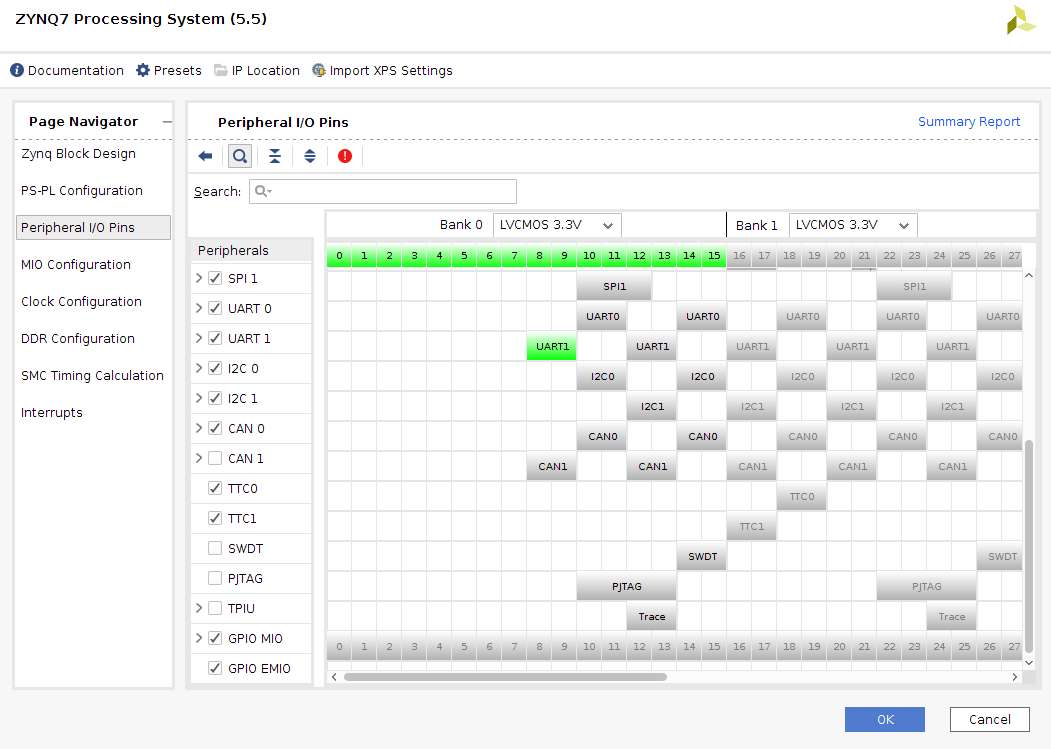
\includegraphics[width=\textwidth]{can-enable.png}
				\caption{Vivado project - IP Core configuration.}\label{fig:can-enable}
			\end{figure}
		\end{column}
		\begin{column}{0.5\textwidth}
			\begin{itemize}
				\item Apply the configuration in the TCL script, provided by the manufacturer.
				\item Enable all the required peripherals (CAN, USB, etc).
				\item Route all the enabled modules to an available MIO pin or via EMIO.
				\item Configure the frequency for the CAN REF CLK signal (80 MHz).
			\end{itemize}
		\end{column}
	\end{columns}
\end{frame}

\begin{frame}
	\frametitle{Hardware Project}
	\begin{columns}
		\begin{column}{0.5\textwidth}
			\begin{figure}
				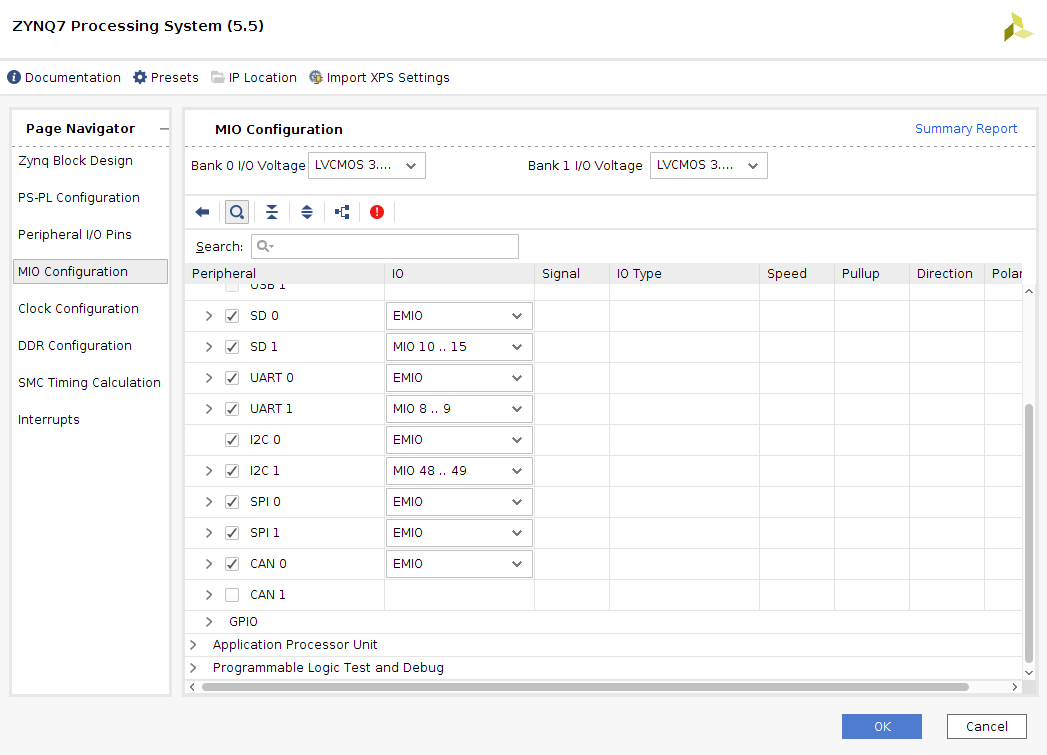
\includegraphics[width=\textwidth]{can-emio.png}
				\caption{Vivado project - Signals routing.}\label{fig:can-emio}
			\end{figure}
		\end{column}
		\begin{column}{0.5\textwidth}
			\begin{figure}
				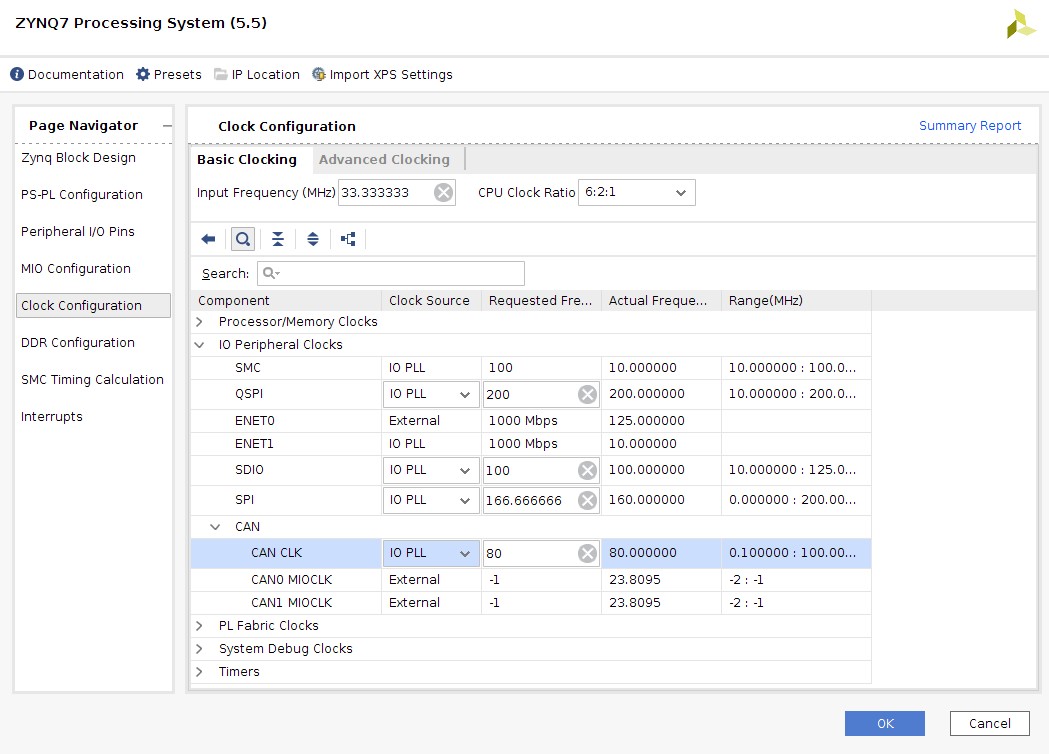
\includegraphics[width=\textwidth]{can-clock.png}
				\caption{Vivado project - Clock configuration.}\label{fig:can-clock}
			\end{figure}
		\end{column}
	\end{columns}
\end{frame}

\begin{frame}
	\frametitle{Hardware Project}
	\begin{columns}
		\begin{column}{0.5\textwidth}
			\begin{figure}
				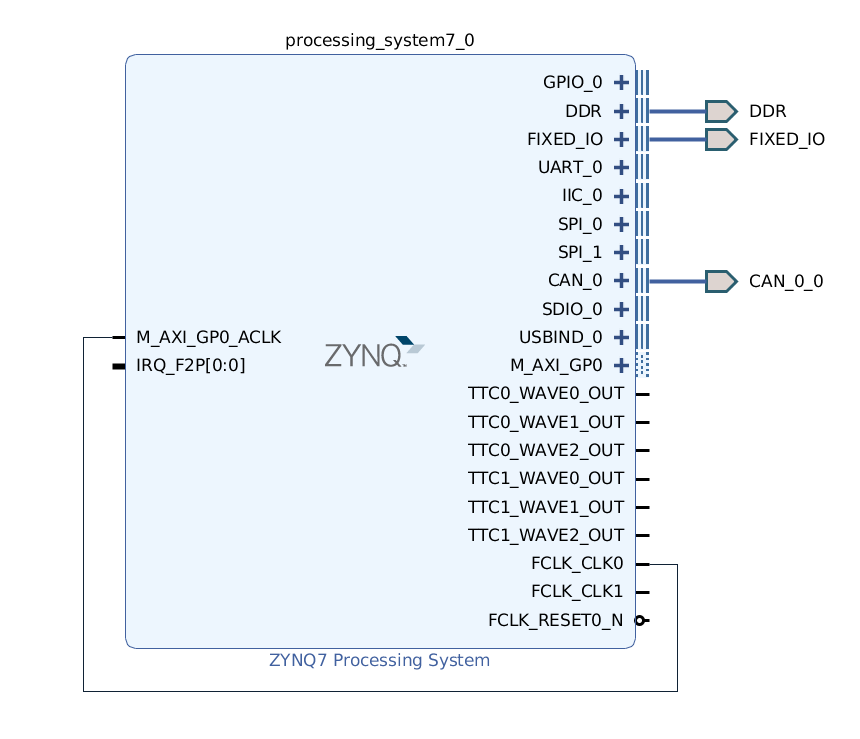
\includegraphics[width=\textwidth]{ip-core.png}
				\caption{Vivado project - Block Design.}\label{fig:ip-core}
			\end{figure}
		\end{column}
		\begin{column}{0.5\textwidth}
			\begin{itemize}
				\item Run the Block Automation wizard.
				\item Run the Connection Automation wizard.
				\item Set all signals that will be routed to a physical pin external (Make external).
				\item Generate an HDL wrapper for the Block Design.
				\item Open the Elaborated Design (RTL Analysis), and set the I/O planning layout.
			\end{itemize}
		\end{column}
	\end{columns}
\end{frame}

\begin{frame}
	\frametitle{Hardware Project}
	\begin{columns}
		\begin{column}{0.5\textwidth}
			\begin{figure}
				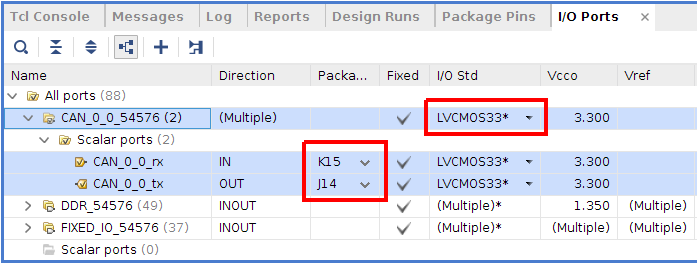
\includegraphics[width=\textwidth]{set-constraints.png}
				\caption{Vivado project - External pins mapping.}\label{fig:set-constraints}
			\end{figure}
		\end{column}
		\begin{column}{0.5\textwidth}
			\begin{itemize}
				\item Config the IO standard and package pin for the external signals (see Trenz TRM \cite{zynq-trm}).
				\item Run Synthesis, Implementation and Generate Bitstream.
				\item Export hardware, including bitstream file.
				\item Launch SDK, selecting the local project environment.
			\end{itemize}
		\end{column}
	\end{columns}
\end{frame}

\begin{frame}
	\frametitle{Hardware Project}
	\begin{columns}
		\begin{column}{0.5\textwidth}
			\begin{figure}
				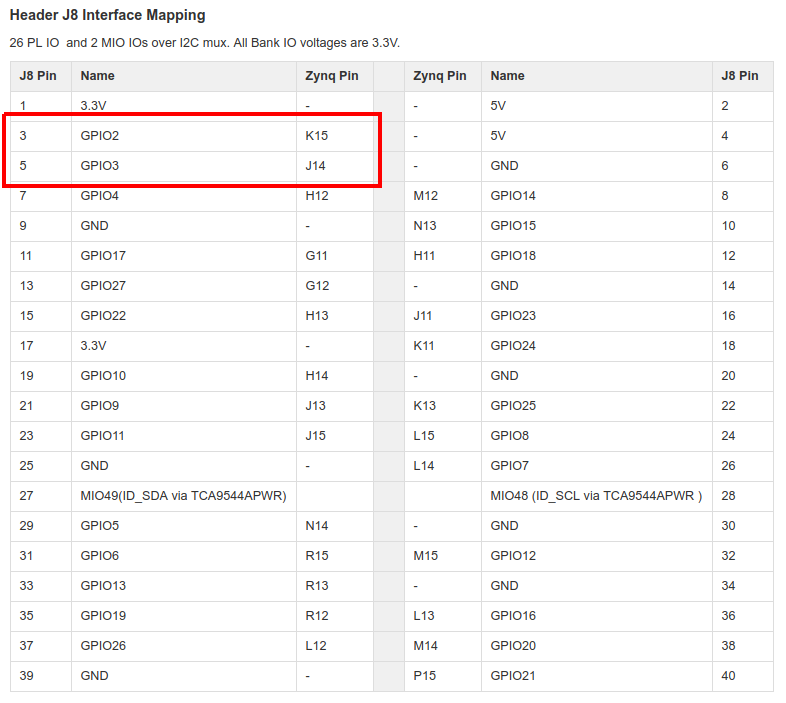
\includegraphics[width=\textwidth]{zynq-pins.png}
				\caption{Vivado project - Mapped pins location.}\label{fig:zynq-pins}
			\end{figure}
		\end{column}
		\begin{column}{0.5\textwidth}
			\begin{figure}
				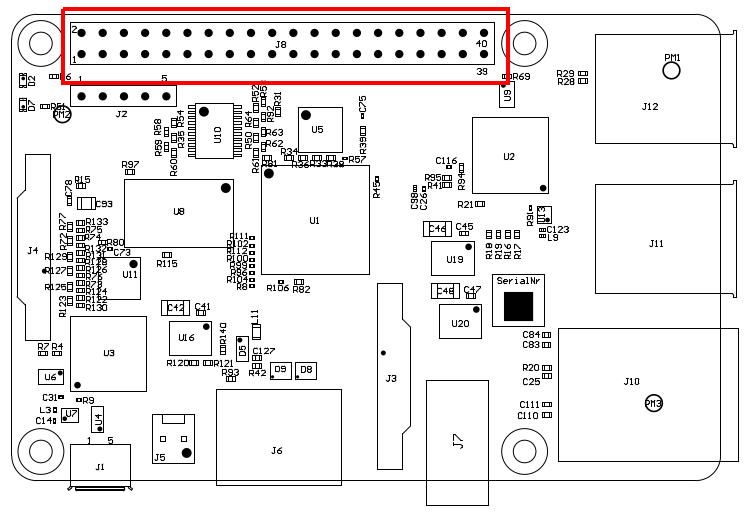
\includegraphics[width=\textwidth]{header-pins.png}
				\caption{Vivado project - Header pins identification.}\label{fig:header-pins}
			\end{figure}
		\end{column}
	\end{columns}
\end{frame}

\begin{frame}[fragile]
	\frametitle{GUI Vs. TCL Console}
	Vivado includes a TCL scripting language integrated, for more complex designs. The entire GUI interaction can be translated into TCL command.
	\lstinputlisting[language=tcl, basicstyle=\tiny\ttfamily, tabsize=2, commentstyle=\color{darkgray}, keywordstyle=\color{blue}, backgroundcolor=\color{lightgray}, morekeywords={create_project, create_bd_design, update_compile_order, create_bd_cell, apply_bd_automation}, firstline=1, lastline=10, breaklines=true, numbers=left]{../../../git/DAEbot/Devices/Zynqberry_OperatorPlus/zynqberryHW_CAN/create_project.tcl}
\end{frame}

\subsection{Xilinx SDK}

\begin{frame}
	\frametitle{Software Project}
	Based on the Eclipse SDK, for application development on Zynq Ultrascale+ MPSoC and Zynq-7000 All Programmable families.
	\vfill
	\begin{columns}
		\begin{column}{0.5\textwidth}
			\begin{itemize}
				\item Editor
				\item Compilers
				\item Build tools
				\item Flash memory Management
				\item JTAG debug integration
			\end{itemize}
		\end{column}
		\begin{column}{0.5\textwidth}
			\begin{itemize}
				\item Hierarchical Profiling
				\item Bare-Metal and Linux development
				\item Homogeneous and heterogeneous multi-processor support
			\end{itemize}
		\end{column}
	\end{columns}
\end{frame}

\begin{frame}
	\frametitle{Software Project structure}
	\begin{columns}
		\begin{column}{0.5\textwidth}
			\begin{figure}
				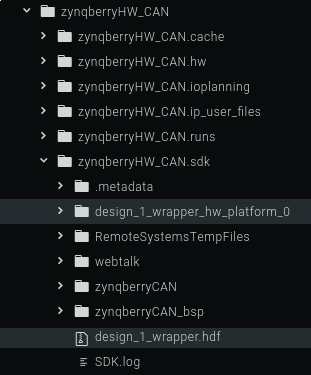
\includegraphics[width=0.8\textwidth]{xilinx-project-structure.png}
				\caption{Xilinx SDK project structure.}\label{fig:xilinx-project-structure}
			\end{figure}
		\end{column}
		\begin{column}{0.5\textwidth}
			\begin{block}{Design aware}
				The software project is handled inside the Vivado project environment, and asimilates the Hardware design to configure Software parameters.
			\end{block}
		\end{column}
	\end{columns}
\end{frame}

\begin{frame}
	\frametitle{Software Project structure}
	\begin{columns}
		\begin{column}{0.5\textwidth}
			\begin{figure}
				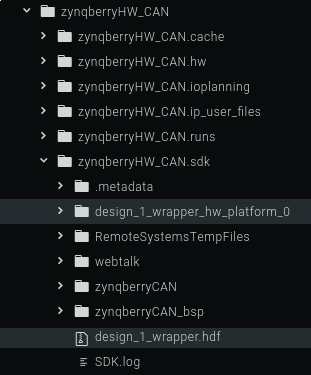
\includegraphics[width=0.8\textwidth]{xilinx-project-structure.png}
				\caption{Xilinx SDK project structure.}\label{fig:xilinx-project-structure}
			\end{figure}
		\end{column}
		\begin{column}{0.5\textwidth}
			\begin{block}{Design aware}
				The software project is handled inside the Vivado project environment, and asimilates the Hardware design to configure Software parameters.
			\end{block}
		\end{column}
	\end{columns}
\end{frame}

\begin{frame}
	\frametitle{Integration issue}
	When the hardware project is exported and SDK is launched with the workspace local to the hardware project, The SDK folder gets linked to the hardware platform designed.
	\vfill
	\begin{alertblock}{Duplicate files/folers alert}
		If a change is made in the hardware project \textbf{after} the SDK project is created, Vivado will create a second hardware platform into SDK. Care need to be taken regardless hardware version, and duplicate files.
	\end{alertblock}
\end{frame}

\section{Application}
% Chapter 1 (from pres-main tex file)
% New Trends in Research
% Author: Javier Reyes

\subsection{Design}



\subsection{Results}



\begin{frame}[standout]
	Thank you!
\end{frame}

% References
\begin{frame}[allowframebreaks]{References}
	\printbibliography
	\nocite{*}
\end{frame}

\end{document}
	